%=================
%textury

\section{Generování textur}
\label{sec:texture}
Textura slouží pro detailní popis struktury povrchu.
Vyskytují se nejčastěji ve formě dvojrozměrných obrázků.
Můžeme se ale setkat i s jednorozměrnými, trojrozměrnými nebo dokonce čtyřrozměrnými texturami.
Trojrozměrné textury slouží pro popis objemu a čtyř\-roz\-měr\-né pro popis objemu měnícího se v čase (například plameny ohně, kouř).
Textury si díky jejich velikosti nemůžeme do programu uložit, a tak je musíme generovat.
Vytvoření textury bývá obvykle časově náročné, neboť obsahují velké množství dat.
Základem pro vytvoření textur v této prací je šum, který je popsaný v části \ref{sec:sum} a vzdálenostního pole vytvořené z Voroného diagramu, který je popsaný v části \ref{sec:voronoid}.
Tyto dvě metody nám produkují $d$ rozměrné pole.
Všechny hodnoty těchto polí jsou v rozsahu $\langle 0,1 \rangle$.
Příklad šumu můžeme vidět v pravé části obrázku \ref{fig:sum} a příklad vzdálenostního pole v pravé části obrázku \ref{fig:voronoid}.
Nejdůležitějším vstupem algoritmu pro vytvoření šumu je faktor vyhlazení, který nám určuje poměr nízkých frekvencí a vysokých frekvencí ve výsledném šumu.
U Voroného diagramu je nejdůležitějším vstupem rozmístění a počet středů buněk.
Nicméně tyto možnosti nám neposkytují dos\-ta\-teč\-nou variabilitu textur.
Proto je vhodné pole hodnot produkované těmito postupy ještě dále upravit.
Upravit takové pole můžeme prostým obarvením pomocí barevného přechodu, globální transformací jako je například vyhlazení, lokální transformací a složením několika vstupů.
Jednotlivé úpravné operace si popíšeme v dalších částech práce.

\subsection{Barevné přechody}
Příklad barevného přechodu je zobrazen na obrázku \ref{fig:prechod}.
Barevný přechod (nebo též gradient) jsou v podstatě tři funkce $R(x),G(x),B(x)$ (čtyři v případě přítomnosti alfa kanálu).
Tyto funkce jsou definované na intervalu $\langle 0,1 \rangle$.
Jejich vstup je hodnota celkové intenzity barvy a výstupem intenzita červené respektive zelené respektive modré barvy.
Intenzity jsou taktéž v rozsahu $\langle 0,1 \rangle$.
Barevné přechody můžeme výhodně použít na obarvení obrázků v odstínech šedé.
Znázorněné to můžeme vidět na obrázku \ref{fig:gradmap}.
Pro uložení barevného přechodu stačí uložit jen kontrolní barvy a hodnoty mezi nimi interpolovat.
Například u barevného přechodu na Obrázek \ref{fig:prechod} stačí uložit pouze barvy: tmavě modrá, světle modrá, žlutá, světle zelená, tmavě zelená, šedá a bílá (v pořadí zleva doprava).
Tímto můžeme zredukovat paměťovou náročnost.
Další možností je vytvořit algoritmus na generování barevných přechodů.
Musíme však zvážit, jestli potřebujeme tolik různých barevných přechodů, že se nám je oplatí generovat.

\begin{figure}[h]
\centering

\includegraphics[width=15cm,keepaspectratio]{obr/gradient.png}
\caption{Barevný přechod, který je možné využít na obarvení výškové mapy.}
\label{fig:prechod}
\end{figure}

\begin{figure}[h]
\centering
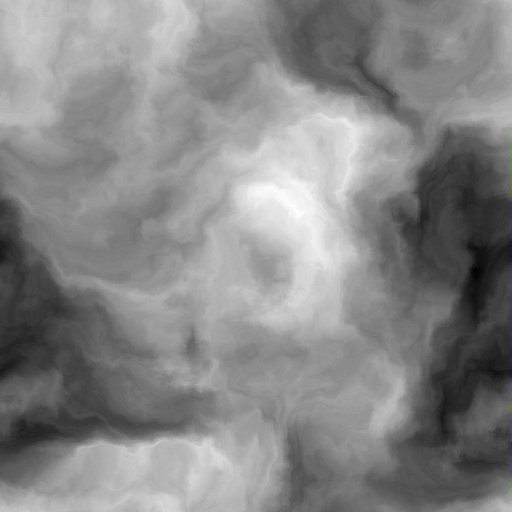
\includegraphics[width=7.5cm,keepaspectratio]{obr/gradmap0.jpg}
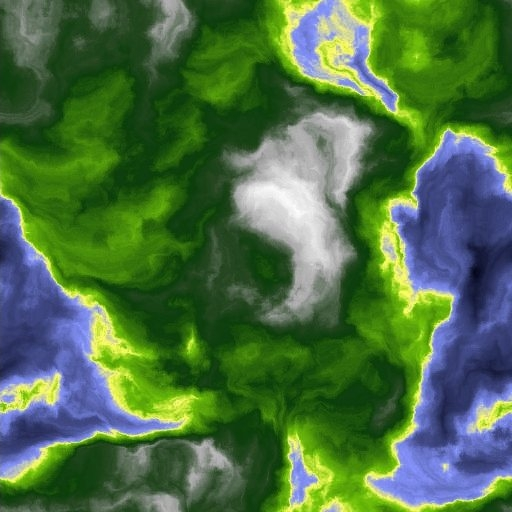
\includegraphics[width=7.5cm,keepaspectratio]{obr/gradmap1.jpg}
\caption{Vlevo: vstupní obrázek v odstínech šedé. Vpravo: obarvený obrázek z leva barevným přechodem z obrázku \ref{fig:prechod}}
\label{fig:gradmap}
\end{figure}

\subsection{Globální transformace}
Globální transformací budeme v textu rozumět operaci, která transformuje vstupní $d$ roz\-měr\-né pole hodnot na výstupní $d$ rozměrné pole hodnot.
Pro výpočet jednoho prvku výstupního pole s indexem $I$ budeme potřebovat hodnoty okolí vstupního pole kolem indexu $I$.
Jedná se tedy o $d$ rozměrnou konvoluci s $d$ rozměrným konvolučním jádrem.
Pokud si vytvoříme obecnou konvoluci, můžeme ji použít pro řadu transformací.
Příkladem těchto transformací je vyhlazení a detekce hran.
Konvoluční jádro pro vyhlazení obsahuje hodnoty, které jsou všechny stejné a jejichž součet je roven jedné.

\subsection{Lokální transformace}
Lokální transformací budeme v textu rozumět (podobně jako globální transformace) operaci, která transformuje vstupní pole na výstupní pole hodnot.
Pole mají rozměr $d$.
Pro výpočet jednoho prvku výstupního pole s indexem $I$ budeme potřebovat několik hodnot ze vstupního pole.
Výběr těchto hodnot závisí na transformaci.
%Příklady lokálních transformací vzdálenostního pole můžeme vidět na Obrázek 3.15 až Obrázek 3.26.
Možnosti lokální transformace jsou velké.
Vše závisí na transformační funkci.
Důležité je, aby nám transformace zachovávala opakování.
Kdykoliv si transformace zažádá  hodnotu pole na souřadnicích, které leží mimo rozsah pole, budeme muset souřadnice přepočítat.
Souřadnice bodu pole je $I=(i_1,i_2,\dotsc,i_d)$ a velikost pole (výška, šířka, ...) je $r=(r_1,r_2,\dotsc,r_d)$.
Pokud je složka souřadnic $i_n<0 \vee i_n \geq r_n$ (hodnoty pole indexujeme od nuly), je potřeba ji přepočítat podle vztahu: $i'_n= ((i_n \% r_n)+r_n)\% r_n$.

V levé části obrázku \ref{fig:voropopis} můžeme vidět velmi jednoduchou transformaci.
K výpočtu výstupní hodnoty na souřadnicích $I=(i_1,i_2)$ jsou zapotřebí dvě hodnoty vstupního pole.
První hodnota vstupního pole, označme ji $a$ , je na totožných souřadnicích.
Druhá hodnota, označme ji $b$, je na souřadnicích $(i_1 + r\cdot \cos(2\pi a),i_2+r\cdot \sin(2\pi a))$.
Hodnota $r$ udává poloměr.
Hodnota $b$ je výsledná hodnota výstupního pole na souřadnicích $I$.
Můžeme vidět, že hodnota $a$ udává normalizovaný úhel.
Spolu s poloměrem $r$ vytváří vektor.
Když tento vektor přičteme k původním souřadnicím, máme souřadnice bodu, jehož hodnota je použita pro výstup – tedy hodnotu $b$.
Na dalších obrázcích je postup transformace obdobný.
V pravé části obrázku \ref{fig:voropopis} je výše popsaný postup opakován několikrát.
Místo abychom použili dva body ze vstupního pole, použijeme jich několik.
Poslední bod udává hodnotu výstupu.
Další příklady lokálních transformací můžeme vidět na obrázku \ref{fig:loctransform}

\begin{figure}[h]
\centering
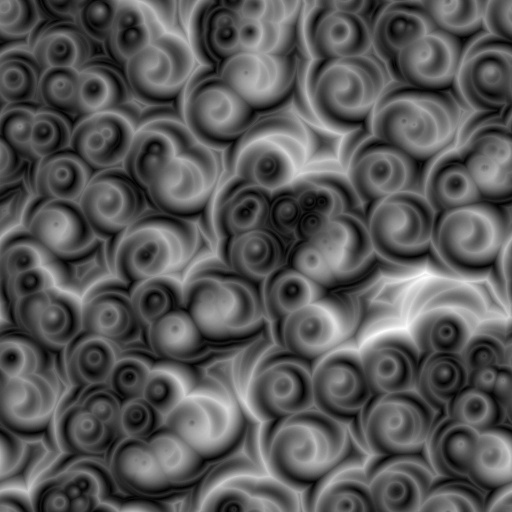
\includegraphics[width=7.5cm,keepaspectratio]{obr/voro_00.jpg}
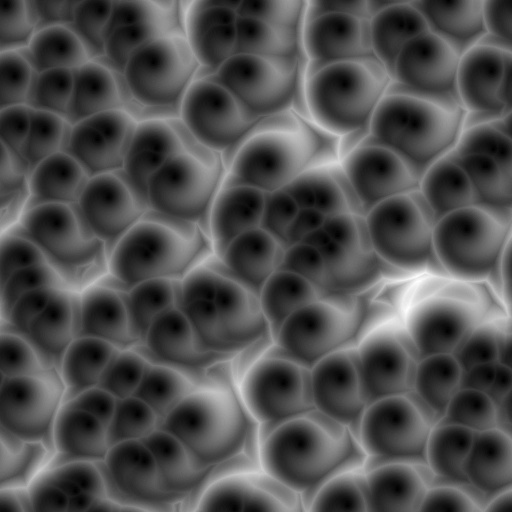
\includegraphics[width=7.5cm,keepaspectratio]{obr/voro_01.jpg}
\caption{Lokální transformace}
\label{fig:voropopis}
\end{figure}


\subsection{Skládání operací}
Nyní, když máme základ všech textur v podobě distančního pole a šumu, lokální a globální transformace a barevné přechody, můžeme se pustit do vytváření textur.
Vytvoření jedné textury si můžeme představit jako strom.
Uzly stromu představují operaci.
Operace uložena v uzlu bere své vstupy ze svých potomků a výstup posílá rodiči.
V listech tohoto stromu se nachází buď distanční pole nebo šum.
V uzlech stromu je lokální nebo globální transformace nebo jedna z následujících operací:
\begin{itemize}
\item
Součet hodnot vstupů.
\item
Rozdíl hodnot vstupů.
\item
Násobení hodnot vstupů.
\item
Součet hodnot vstupů s ohledem na alfa kanál.
\item
Kompozice vstupů do vícekanálové textury.
\end{itemize}
Příklad textury složené pomocí několika operací můžeme vidět na obrázku \ref{fig:slozenina}

\begin{figure}[h]
\centering
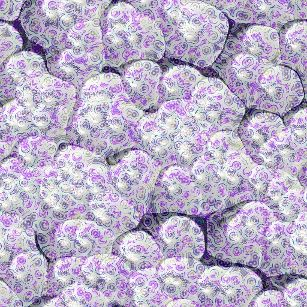
\includegraphics[width=7.5cm,keepaspectratio]{obr/slozeni.jpg}
\caption{Sestavená textura}
\label{fig:slozenina}
\end{figure}

\begin{figure}[htb]
\centering
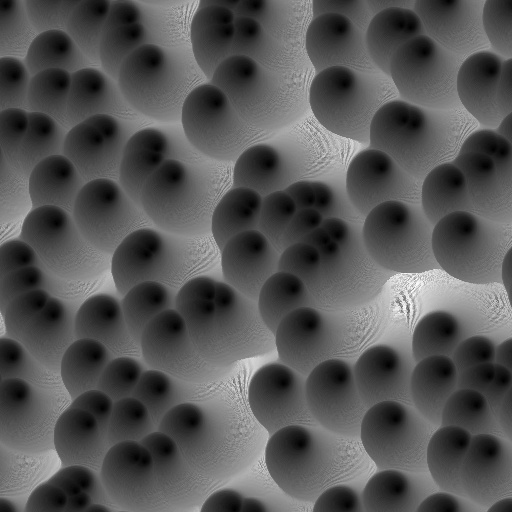
\includegraphics[width=3cm,keepaspectratio]{obr/voro_02.jpg}
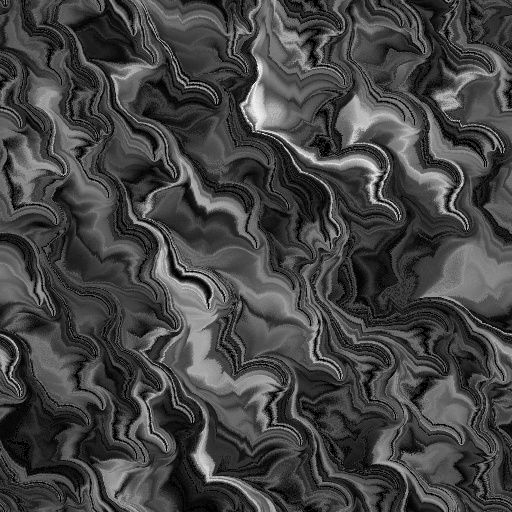
\includegraphics[width=3cm,keepaspectratio]{obr/voro_03.jpg}
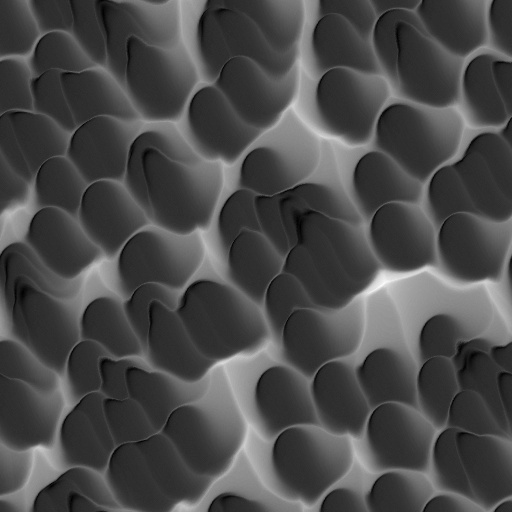
\includegraphics[width=3cm,keepaspectratio]{obr/voro_04.jpg}
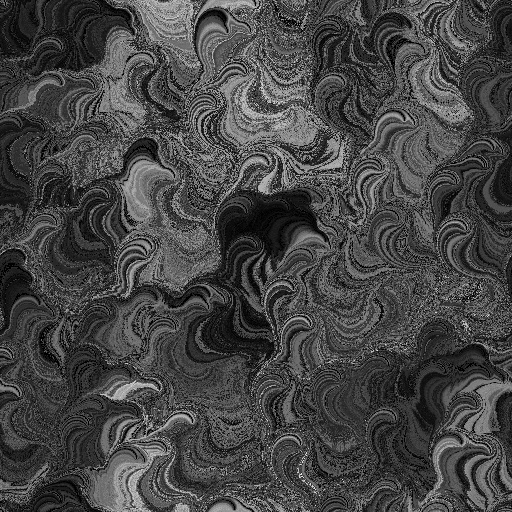
\includegraphics[width=3cm,keepaspectratio]{obr/voro_05.jpg}
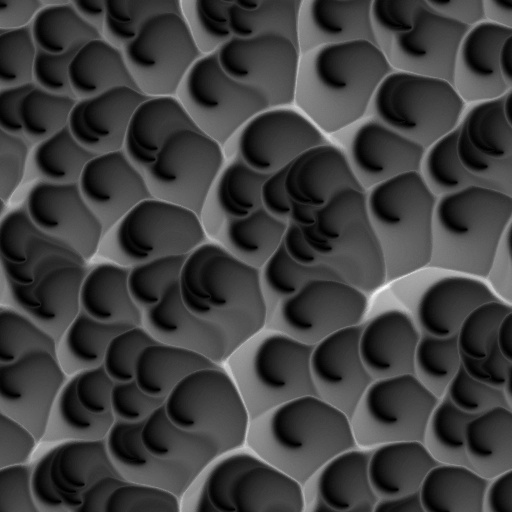
\includegraphics[width=3cm,keepaspectratio]{obr/voro_06.jpg}
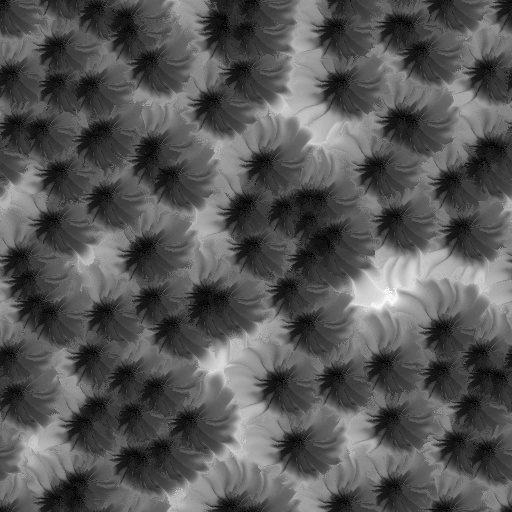
\includegraphics[width=3cm,keepaspectratio]{obr/voro_07.jpg}
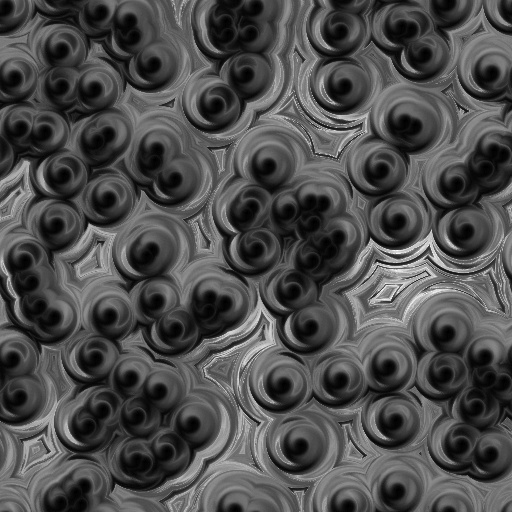
\includegraphics[width=3cm,keepaspectratio]{obr/voro_08.jpg}
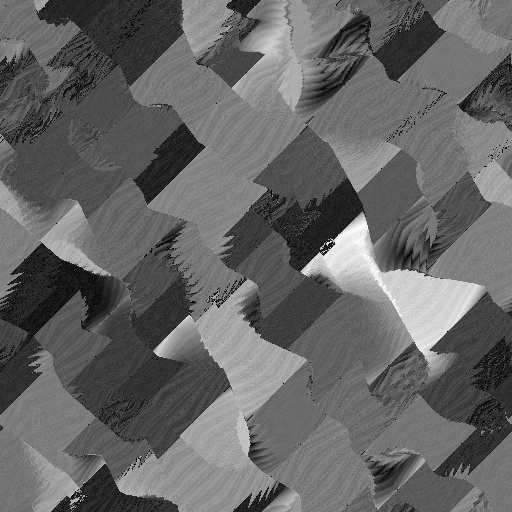
\includegraphics[width=3cm,keepaspectratio]{obr/voro_09.jpg}
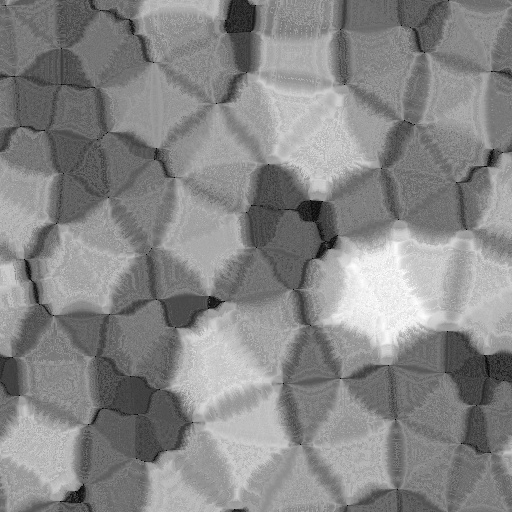
\includegraphics[width=3cm,keepaspectratio]{obr/voro_10.jpg}
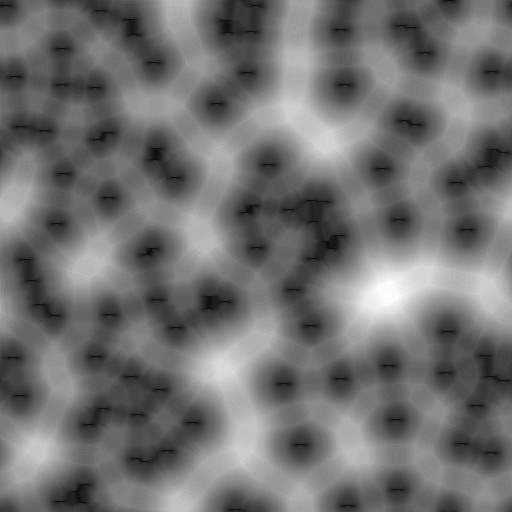
\includegraphics[width=3cm,keepaspectratio]{obr/voro_11.jpg}
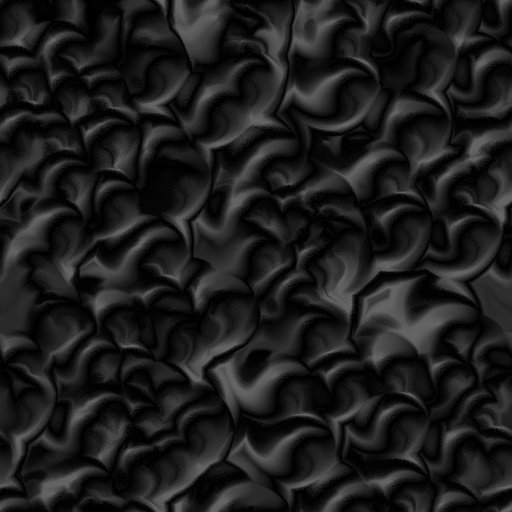
\includegraphics[width=3cm,keepaspectratio]{obr/voro_12.jpg}
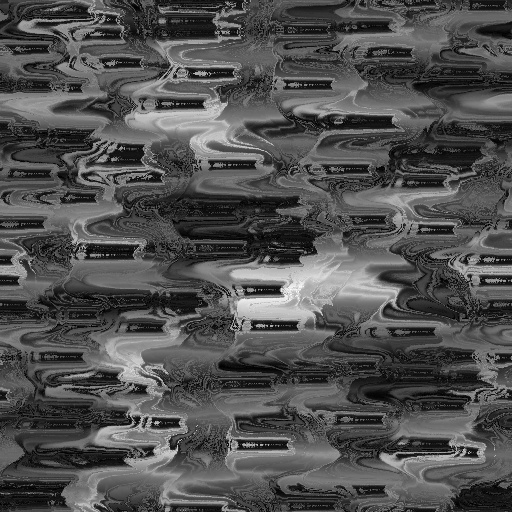
\includegraphics[width=3cm,keepaspectratio]{obr/voro_13.jpg}
\caption{Příklady lokálních transformací aplikovaných na vzdálenostní pole.}
\label{fig:loctransform}
\end{figure}

